%%%%%%%%%%%%%%%%%%%%%%%%%%%%%%%%%%%%%%%%%%%%%%%%%%%%%%%%%%%
% --------------------------------------------------------
%  _____
% |_   _|_ _ _   _
%   | |/ _` | | | |
%   | | (_| | |_| |
%   |_|\__,_|\__,_|
%
% LaTeX2e Template
% Version 2.6.0 (21/04/2026)
%
% Original template author:
% Guillermo Jimenez (memo.notess1@gmail.com)
%
% License:
% Creative Commons CC BY 4.0
% --------------------------------------------------------
%%%%%%%%%%%%%%%%%%%%%%%%%%%%%%%%%%%%%%%%%%%%%%%%%%%%%%%%%%%

\documentclass[9pt,a4paper,twocolumn,twoside]{tau-class/tau}
\usepackage[english]{babel}

%----------------------------------------------------------
% Title & Authors/Affiliations
%----------------------------------------------------------

\doctype{Cloud Computing and Distributed Systems}
\title{Project report for an AWS multiplayer matchmaking engine}

\author[a,1]{Alessandro Fantesini\thanks{\href{mailto:alessandro.fantesini@student.unibz.it}{alessandro.fantesini@student.unibz.it}}}
\author[b,2]{Antonia Stieger\thanks{\href{mailto:antonia.stieger@student.unibz.it}{antonia.stieger@student.unibz.it}}}
\author[c,3]{Ondrej M\"uller\thanks{\href{mailto:ondrej.mueller@student.unibz.it}{ondrej.mueller@student.unibz.it}}}

\affil[a]{Free University of Bozen-Bolzano, Italy}
\affil[b]{Free University of Bozen-Bolzano, Italy}
\affil[c]{Free University of Bozen-Bolzano, Italy}

\footinfo{AWS Multiplayer Matchmaking Engine}
\theday{\today}
\organization{Free University of Bozen-Bolzano}
\leadauthor{Fantesini, Stieger, M\"uller}

%----------------------------------------------------------
% Abstract and Keywords
%----------------------------------------------------------

\begin{abstract}
    This project studies how a cloud-based backend can support multiplayer game matchmaking. Our main question was: can we build a small but realistic matchmaking engine that authenticates players, groups them by skill, and assigns them to a running game server while keeping the infrastructure mostly serverless and easy to deploy? To answer this, we implemented an AWS system. Players create matchmaking tickets through a REST API, a scheduled matchmaker groups compatible tickets using an Elo-based rule, and each successful group receives the address of a Red Eclipse dedicated server running in a Docker container.

    The project was partly inspired by an online tutorial video \cite{youtubeMatchmakingVideo} about building multiplayer game infrastructure on AWS, but we adapted the idea to our own simpler architecture because of the limits introduced by the AWS Academy Learner Lab. We tested the system with individual end-to-end tests, an eight-player group test, and a benchmark for starting game servers on ECS/EC2. The implementation showed that a serverless design is a good fit for the ticketing and polling part of matchmaking, while the actual game server still needs long-running compute. The main tradeoff we observed is between simplicity and responsiveness: a scheduled Lambda is easy to operate, but server allocation can still create visible waiting time.
\end{abstract}

\keywords{cloud computing, distributed systems, multiplayer games, matchmaking, AWS, serverless}

\begin{document}

    \maketitle
    \thispagestyle{firststyle}

%----------------------------------------------------------

\section{Introduction}

    \taustart{T}he main idea of our project was to build the backend part of a multiplayer game matchmaking system in the cloud. In many online games, the player does not manually choose a server from a list. Instead, the player presses a button, waits in a queue, and the game backend finds other players with a similar level before sending everyone to a game server. This seems simple from the player's point of view, but it involves several distributed-system problems: authentication, shared state, queue management, fairness, server allocation, scaling, failures, and latency.

    The questions we tried to answer were: \textit{how can we implement a cloud-based matchmaking engine that best balances the time players spend in the queue waiting and the fairness of the match? What is the best solution from a performance and price point of view regarding the size of the EC2 instances?} 
    
    We focused on a session-based game model. A player has a profile with an Elo rating, starts matchmaking through an authenticated API call, and receives a ticket. A background process periodically scans all waiting tickets. If enough players are waiting and their Elo values are close enough, they are grouped into one match. The system then assigns them to a running Red Eclipse game server container and provides the player with the server IP address and UDP port.

    We did not try to build a complete commercial system. 
    The goal was instead to understand the infrastructure pattern: how a cloud backend can move from ``player wants a match'' to ``player has a server to connect to''.

\section{Related Work}

    Matchmaking has two major goals that often conflict: matches should be found quickly, but they should also be good matches. The meaning of ``good'' depends on the game. For a competitive game it may mean similar skill. For a fast action game it may mean low latency. 
    Amazon GameLift FlexMatch \cite{awsFlexMatch2017,awsFlexMatch2024} describes this as a rule-based matching problem where developers define attributes such as skill or latency, then relax rules as players wait longer. This idea influenced our implementation: our matchmaker starts with a strict Elo tolerance and then widens the tolerance over time.

    League of Legends is a useful example of this tradeoff from an existing game. Riot describes its matchmaking as trying to balance fair matches, position preferences, and quick queues \cite{riotLeagueMatchmaking}. The exact system is much more complex than ours, but the basic problem is similar: if the system waits too long it becomes frustrating, while if it accepts a match too quickly the result may feel unfair. This helped us frame our own simplified version as a balance between Elo fairness, queue time, and latency.

    Skill-based matchmaking is strongly connected to rating systems. The classic starting point is Elo's rating system \cite{elo1978rating} for chess. Elo represents player skill as one number, which makes it very convenient for a small project like ours. 
    We chose a simple Elo value because our main contribution was the cloud infrastructure.

    Another important research direction is latency-aware matchmaking. Agarwal and Lorch \cite{agarwal2009matchmaking} studied matchmaking for online games and other latency-sensitive peer-to-peer systems using a very large trace from Xbox players. Their work shows that players care strongly about lag and that matchmaking can benefit from latency prediction rather than measuring every possible connection at queue time. Our project did not implement latency-based region selection, but this paper is relevant because it explains a limitation of our design: two players with similar Elo values might still have a bad experience if they are far away from the server or from each other.

    We also looked at cloud game hosting ideas from AWS. GameLift is the managed AWS service for dedicated session-based game servers, and FlexMatch can be connected to game session queues. We could not use GameLift directly due to the AWS Academy Learner Lab constraints. Instead, we recreated a smaller version with API Gateway, Lambda, DynamoDB, and ECS. 
    The YouTube video \cite{youtubeMatchmakingVideo} we came across during the topic search was useful as a practical inspiration for how cloud services can be combined for game backend workflows. Our final design is simpler than a managed GameLift architecture, but it follows the same broad separation between matchmaking logic and game-server hosting.

\section{Infrastructure and Application Design}

    The system is deployed with AWS SAM \cite{awsSamDocs}, so the infrastructure is defined as code in \inlinecode{template.yaml}. SAM is built on CloudFormation and gives a shorter syntax for serverless resources such as Lambda functions and API Gateway routes. This was useful because we had to redeploy often while developing.

    The application has five main parts. First, Amazon Cognito manages users and creates JSON Web Tokens (JWT). Second, API Gateway exposes REST endpoints and validates those JWTs. Third, Lambda functions implement the application logic. Fourth, DynamoDB stores player profiles and matchmaking tickets. Finally, ECS on EC2 runs the actual Red Eclipse server containers.

    The REST API contains these main endpoints:

    \begin{itemize}
        \item \inlinecode{POST /register}: create a Cognito user and a player profile.
        \item \inlinecode{POST /match}: create a matchmaking ticket for the authenticated player.
        \item \inlinecode{GET /match/\{ticketId\}}: check whether a ticket is still searching or already matched.
        \item \inlinecode{DELETE /match/\{ticketId\}}: cancel a searching ticket.
        \item \inlinecode{GET /profile}: return the authenticated player's profile.
    \end{itemize}

    The data model is intentionally small. The \inlinecode{PlayerProfiles} table is keyed by the Cognito user ID and stores username, Elo, wins, and losses. The \inlinecode{MatchmakingTickets} table is keyed by ticket ID and stores the user ID, status, Elo, creation time, matched players, server endpoint, ECS task Amazon Resource Name (ARN), and Time-to-Live (TTL). Ticket statuses move through \inlinecode{SEARCHING}, \inlinecode{SUCCEEDED}, \inlinecode{TIMED_OUT}, or \inlinecode{CANCELLED}.

    The most important component is the \inlinecode{MatchStatusPoller} Lambda. 
    EventBridge runs it once per minute. The poller scans all \inlinecode{SEARCHING} tickets, removes tickets older than five minutes by marking them \inlinecode{TIMED_OUT}, sorts active tickets by Elo, and then uses a sliding window to find groups of eight players. The allowed Elo spread starts at 200, increases to 400 after one minute, and increases to 800 after two minutes. This is a simple version of matchmaking rule relaxation.

    After a valid group is found, the poller allocates a game server. ECS maintains a warm pool of Red Eclipse containers. Each container exposes UDP port 26000 internally, but uses dynamic host port mapping, so Docker assigns a random public UDP port on the EC2 instance. The Lambda function calls ECS and EC2 APIs to find the running task, the host port, and the public IP address of the EC2 instance. This endpoint is then written back into all tickets in the matched group.

\section{Technologies and Challenges}

    We used DynamoDB because it is serverless, fast for key-value access, and easy to integrate with Lambda. API Gateway and Cognito gave us authentication without building our own login system. ECS, ECR, and EC2 were used for the Red Eclipse server because a dedicated game server is naturally containerized. The frontend is a small static interface, mainly for interacting with the API during demos.

    Another challenge was the difference between matchmaking tickets and real server capacity. It is easy to mark players as matched in DynamoDB, but the match is not useful unless a reachable game server exists. We therefore had to connect the matchmaker to ECS and make sure that a matched group receives a real IP and port. Dynamic port mapping was useful because multiple containers can run on the same small EC2 instance, but it also meant the Lambda function had to inspect ECS task network bindings after allocation.

    A third challenge was working within small cloud resources. The ECS cluster uses \inlinecode{t3.micro} instances, and the task definition gives each Red Eclipse container 128 MB of memory. This is enough for a prototype, but it forced us to think about warm pools, bin-packing, and how many containers can realistically fit on one instance. We also had to balance cost and responsiveness: keeping warm containers ready improves allocation speed but consumes resources even when no players are waiting.

    Finally, the scheduled poller is simple but not perfect. A one-minute EventBridge interval means a player may wait almost a full minute even if enough compatible players are already present. For tests we manually invoke the poller, but in a real system we would probably trigger matching more frequently, use a queue, or use DynamoDB Streams/EventBridge events.

\section{Experiments}

    We tested the project in three steps. The first tests checked the normal API workflow with one or two users: registering, logging in, creating a matchmaking ticket, polling the ticket status, and cancelling a ticket. These tests were useful because many early bugs were not in the matching algorithm itself, but in the connections between Cognito, API Gateway, Lambda, and DynamoDB.

    The second experiment was the eight-player group test. The setup script creates eight Cognito users and DynamoDB player profiles with known Elo values. The test script authenticates all players, submits eight matchmaking requests, invokes the poller, and repeatedly calls \inlinecode{GET /match/\{ticketId\}} until all tickets reach a terminal state. Since the final match size is eight, this was our main functional test for the matchmaking logic.

    The third experiment measured the game-server startup time. For this test we first scaled the Auto Scaling Group down to one EC2 instance. Then the script increased the desired capacity from one to two, waited until the new instance registered in the ECS cluster, started a first Red Eclipse container on it, and finally started a second container on the same instance. The reason for starting two containers was to separate the one-time Docker image pull from the normal container start time.

    We also wanted to evaluate the full matchmaking goal shown in Figure 1: balancing Elo, player waiting time, and network latency. In the final tests we could only measure Elo grouping and waiting time. We could not realistically emulate players connecting from different geographic regions, so we could not measure the real packet round-trip time between remote players and the EC2 game server. Because of this, latency stayed as a design goal instead of a tested matching rule.

    \begin{figure}[h]
        \centering
        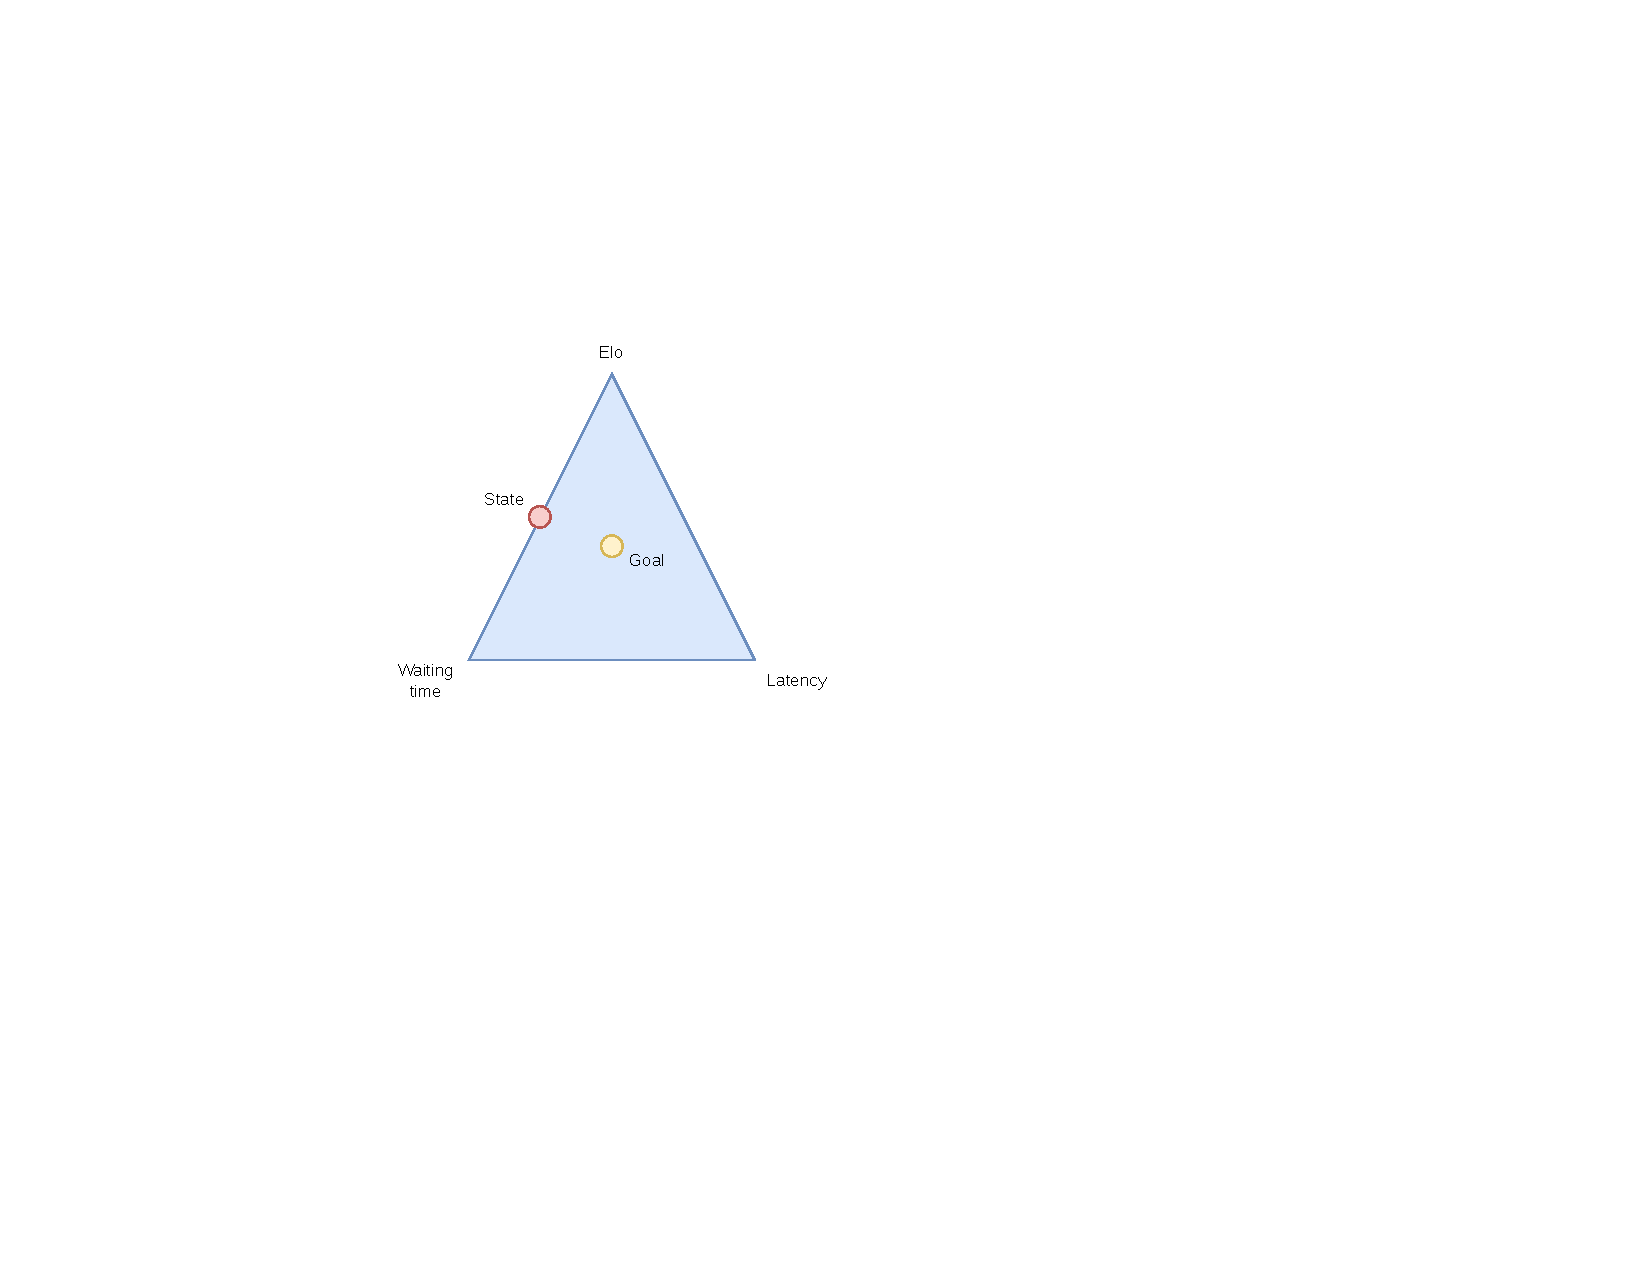
\includegraphics[width=\linewidth]{figures/dia1.pdf}
        \caption{Initial idea for balancing latency, Elo, and waiting time in matchmaking.}
    \end{figure}

\section{Results}

    The functional tests showed that the main workflow works. A player can register, authenticate, create a ticket, and poll it. The matchmaker can group compatible tickets and update them atomically using conditional DynamoDB updates, which prevents overwriting tickets that were cancelled or already changed. In the full-match test, the expected successful result is that both tickets reach \inlinecode{SUCCEEDED} and the API returns the matched players plus the allocated server endpoint.

    The eight-player test is the most representative experiment for our final design because the configured match size is eight. When the eight test players have close enough Elo values, the poller should form exactly one group and assign exactly one ECS server endpoint to all eight tickets. The script also checks for stale \inlinecode{SEARCHING} tickets before running, because old tickets can affect the sorted matching window. This was an important practical lesson: in a stateful distributed system, leftover test data can change the behaviour of later experiments.

    The server startup benchmark gave the most concrete timing result. Creating a new EC2 instance took 40 seconds until it was booted and registered in ECS. Starting the first container on the new instance took 37 seconds. This included pulling the Red Eclipse Docker image from ECR. Starting a second container on the same instance took only 4 seconds because the image was already cached locally.

    This gives two different player experiences. In the normal case, when an instance already exists and the image is cached, a new game server starts in about 4 seconds. In the worst case, when the Auto Scaling Group must create a new instance, the player has to wait about 77 seconds: 40 seconds for EC2 provisioning plus 37 seconds for the first container. From the difference between the first and second container, we estimate that the image pull itself costs about 33 seconds.

    The benchmark also showed a limitation of the \inlinecode{t3.micro} instance. The CPU credit balance before and after the short test was reported as 3.8 credits, which is almost empty for this instance type. Because CloudWatch basic monitoring has a five-minute granularity, this exact number should not be overinterpreted for the short benchmark. Still, together with the previous seven-server load test it suggests that running many game servers on one \inlinecode{t3.micro} can drain CPU credits quickly. Once credits are gone, the instance is limited to its baseline CPU performance, which can cause slower game-server behaviour.

    Overall, the strongest result is that the complete path works: the serverless part can handle the ticket workflow, the poller can create an eight-player match, and ECS can supply a real game-server process. The weakest result is that the system reacts slowly when it has to create completely new compute capacity.

\section{Discussion}

    The project answered the main question partly positively. We were able to build a cloud-based matchmaking engine with realistic components: identity, API, database, background matching, and containerized game servers. The separation of responsibilities is clear, and each AWS service has a specific role. This is a strength of the design because no single component has to do everything.

    At the same time, the implementation also shows why even a small matchmaking system becomes complicated. Our matching logic only uses Elo. This is good for demonstrating skill-based grouping, but it ignores network latency, region, party size, game mode, player behaviour, and server health. In our original plan we wanted to balance Elo, queue time, and latency. In practice we only had one AWS region and no real players connecting from different locations, so we could not collect meaningful latency measurements. This means our final system can form a fair match on paper, but it cannot prove that the selected server would feel good for every player.

    The scheduled polling design is another tradeoff. It is easy to understand, cheap, and reliable for a prototype. However, it adds delay and uses DynamoDB scans, which would not scale well to a very large number of tickets. For this course project, the scheduled Lambda was a reasonable compromise because it made the behaviour easy to test and debug.

    The tests showed that server allocation is the largest practical problem in the current prototype. If capacity is already available, starting another container on a warmed instance took about 4 seconds, which is acceptable for our demo. If a new EC2 instance is needed, the measured wait becomes about 77 seconds. This is too long for a player who has already been told that a match was found. It also shows that matchmaking latency is not only caused by the matching algorithm. The infrastructure state, especially whether an instance is already running and whether the Docker image is cached, matters a lot.

    The \inlinecode{t3.micro} result is another limitation. It is attractive for a student project because it is cheap and fits inside the Learner Lab budget, but the CPU credit balance showed that it is not very robust when many containers are placed on the same machine. A simple improvement for our prototype would be to keep fewer game servers per \inlinecode{t3.micro}, for example three or four instead of seven. Another possible improvement would be to keep a second warmed instance during tests, so the image is already cached and the worst measured wait disappears. These are not complicated architectural changes, but they make the cost and capacity tradeoff more visible.
    
\section{Conclusion}

    In this project we designed and implemented an AWS-based multiplayer matchmaking engine. Players authenticate through Cognito, access the system through API Gateway, create matchmaking tickets, and store state in DynamoDB. A scheduled matchmaker groups players by Elo and assigns each completed match to a Red Eclipse server running in ECS on EC2.

    The project was successful as a prototype because it demonstrates the complete path from user registration to game-server assignment. It also helped us understand the boundary between serverless infrastructure and persistent game-server infrastructure. The main limitations are the simple Elo-only matching model, the one-minute scheduled polling interval, the slow cold start when a new EC2 instance is needed, and the limited CPU headroom of the \inlinecode{t3.micro} instance.

    Without the AWS Learner Lab constraints, we would probably compare our ECS and EC2 pipeline with Amazon GameLift, because GameLift is built specifically for matchmaking and game-server allocation. Additionally, if we had more time, we would add real post-match score reporting and automatic Elo updates. Second, we would include latency or region in the matching rules. Finally, we would replace the scheduled scan with a more event-driven or indexed matchmaking design.

%----------------------------------------------------------

\printbibliography

%----------------------------------------------------------

\end{document}
